\chapter{基于深度学习的用户语义理解方法}

\section{语义理解任务与解决方案描述}
跨界服务平台内服务的智能调用实现过程中,接受的是用户输入的一句有目的性的话,系统在语义理解的过程中,首先要识别用户的意图,对应到系统就是根据
用户意图匹配相应的服务以及匹配该服务要执行的操作,这两者均可被视为分类问题,可以用深度学习的分类算法解决;找到匹配的服务以后,在服务执行前需要
必要的执行参数,可以从用户输入的语句中提取,这将被看作语义槽填充问题,可以用序列标注算法解决,将单词序列x=[$x_{1}$,$x_{2}$,\dots,$x_{T}$]映射到相应的插槽标签序列y=[$y_{1}$,$y_{2}$,\dots,$y_{T}$]。
在本系统中,服务,意图,语义槽(即服务参数)三者具有强相关的关系,

以调用航班信息查询服务为例,来解释跨界服务平台内服务,意图,语义槽(即服务参数)。用户在进入跨界服务平台后,输入“查询成都前往杭州的火车票”,跨界服务平台内
的语义理解模型识别出该语义对应平台内部的<服务>,用户意图为<query查询>,语义槽(即服务参数)为<startCity起始地>成都和<endCity目的地>杭州


\begin{figure}[htbp]
    \centering
    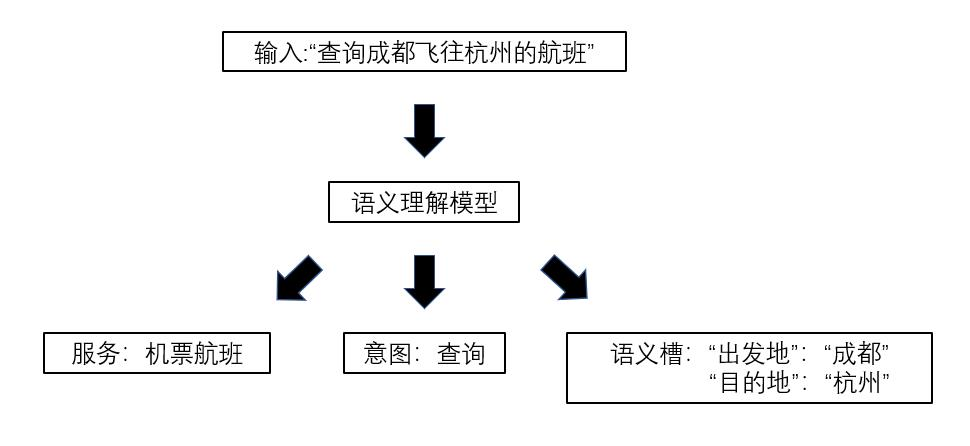
\includegraphics[scale=0.5]{./images/questiondesc.jpg}
    \caption{系统语义理解示例}
    \label{fig:questiondesc}
  \end{figure}


\section{实验预处理}
\subsection{文本分词}
% 结巴分词,word2vec
% 用户不需要输入完整的句子
神经网络的输入是一个向量序列,但用户输入是一个完整的句子,因此首先需要把句子序列化。本文采用结巴分词来做序列化的处理,
结巴分词分了三种模式,准确模式试图将句子切成最准确的句段,适用于文本分析;完全模式会从句子中获取所有可能的单词。 快速但不准确;基于准确模式的搜索引擎模式试图将长词切成几个短词,从而提高查全率。 适用于搜索引擎。
结巴分词的算法依据主要是基于前缀字典结构来实现高效的词图扫描,为所有可能的单词组合构建有向无环图(DAG),使用动态规划根据单词频率查找最可能的组合,对于未知单词,Viterbi算法使用基于HMM的模型来处理。

\begin{table}[htb]
  \centering
  \caption{停用词表}
  \label{tab:RelatedResearchAbroad}
    \begin{tabular}{p{4cm}|p{4cm}|p{6cm}}
      \toprule
      % & \multicolumn{1}{m{60mm}}{\heiti\centering 相关研究成果}
      % \multicolumn{1}{l|}{\heiti 机构名称} & \multicolumn{1}{l|}{\heiti 相关研究内容} & \multicolumn{1}{l}{\heiti 相关研究成果}\\
      % \midrule
      % IBM & 服务科学、服务工程;\\
      % IBM & 服务科学、服务工程;& 提出了服务计算研究框架、服务科学、管理与工程体系\\ \hline
      
      \bottomrule
    \end{tabular}
\end{table}

\subsection{标签的向量化表示}

\section{基于attention-CNN-LSTM的服务分类模型}
实现服务智能调用的第一步要根据用户意图匹配相应的服务,这可以被转化为文本分类问题。
LSTM
是一种特殊的RNN,能够学习长期依赖关系,理解关键字出现的顺序,擅长处理文本序列的问题,同时,
它通过增加门机制来过滤信息,解决了长距离依赖的问题。 另一方面,在某种程度上也避免了梯度消失和梯度爆炸的问题。
CNN
多用于图像领域,由于卷积核的存在,能够提取出词与词之间的隐藏的语义信息,捕获局部相关性。
尽管CNN可以在许多任务中很好地表现,但它最大问题之一是卷积核大小的在训练时固定,不具有很好的泛化能力,一方面,无法对更长的序列信息进行建模,
另一方面,超参数卷积核大小的调整也增加了工作量,Max pooling丢失了结构性信息,因此很难在文本中发现复杂的模式。
为了
能让卷积层从单词嵌入向量中提取更高级别的短语表示,我们在模型中引入attention层.这是因为在传统的CNN中,有效地编码长期上下文信息和非连续词之间的相关性并不容易,
它仅考虑在表面字符串上连续的连续n-gram,因此忽略了非连续词之间的某些长距离相关性,而这种相关性在许多语言中都起着重要作用。比如,用户输入“帮我挂
明天上午邵逸夫医院的号”,这里“挂”和“号”显然应该组合在一起成词才能具有完整正确的语义信息。同时,NLP中有关注意力的大多数现有研究都集中在对不同模式之间的相关性进行建模,
例如机器翻译中源语言和目标语言之间的单词对齐以及问答中问题与答案之间的单词相似性。在本文中,我们将attention层放在卷积层之前,
注意力机制用于自动捕获长期上下文信息和非连续词之间的相关性,而无需任何外部语法信息。

综上所述本节将三者结合各取所长, 采用ATT-CNN-LSTM模型\ref{fig:cnn-lstm}用以解决服务分类问题,下面将详细介绍该模型

\begin{figure}[htbp]
    \centering
    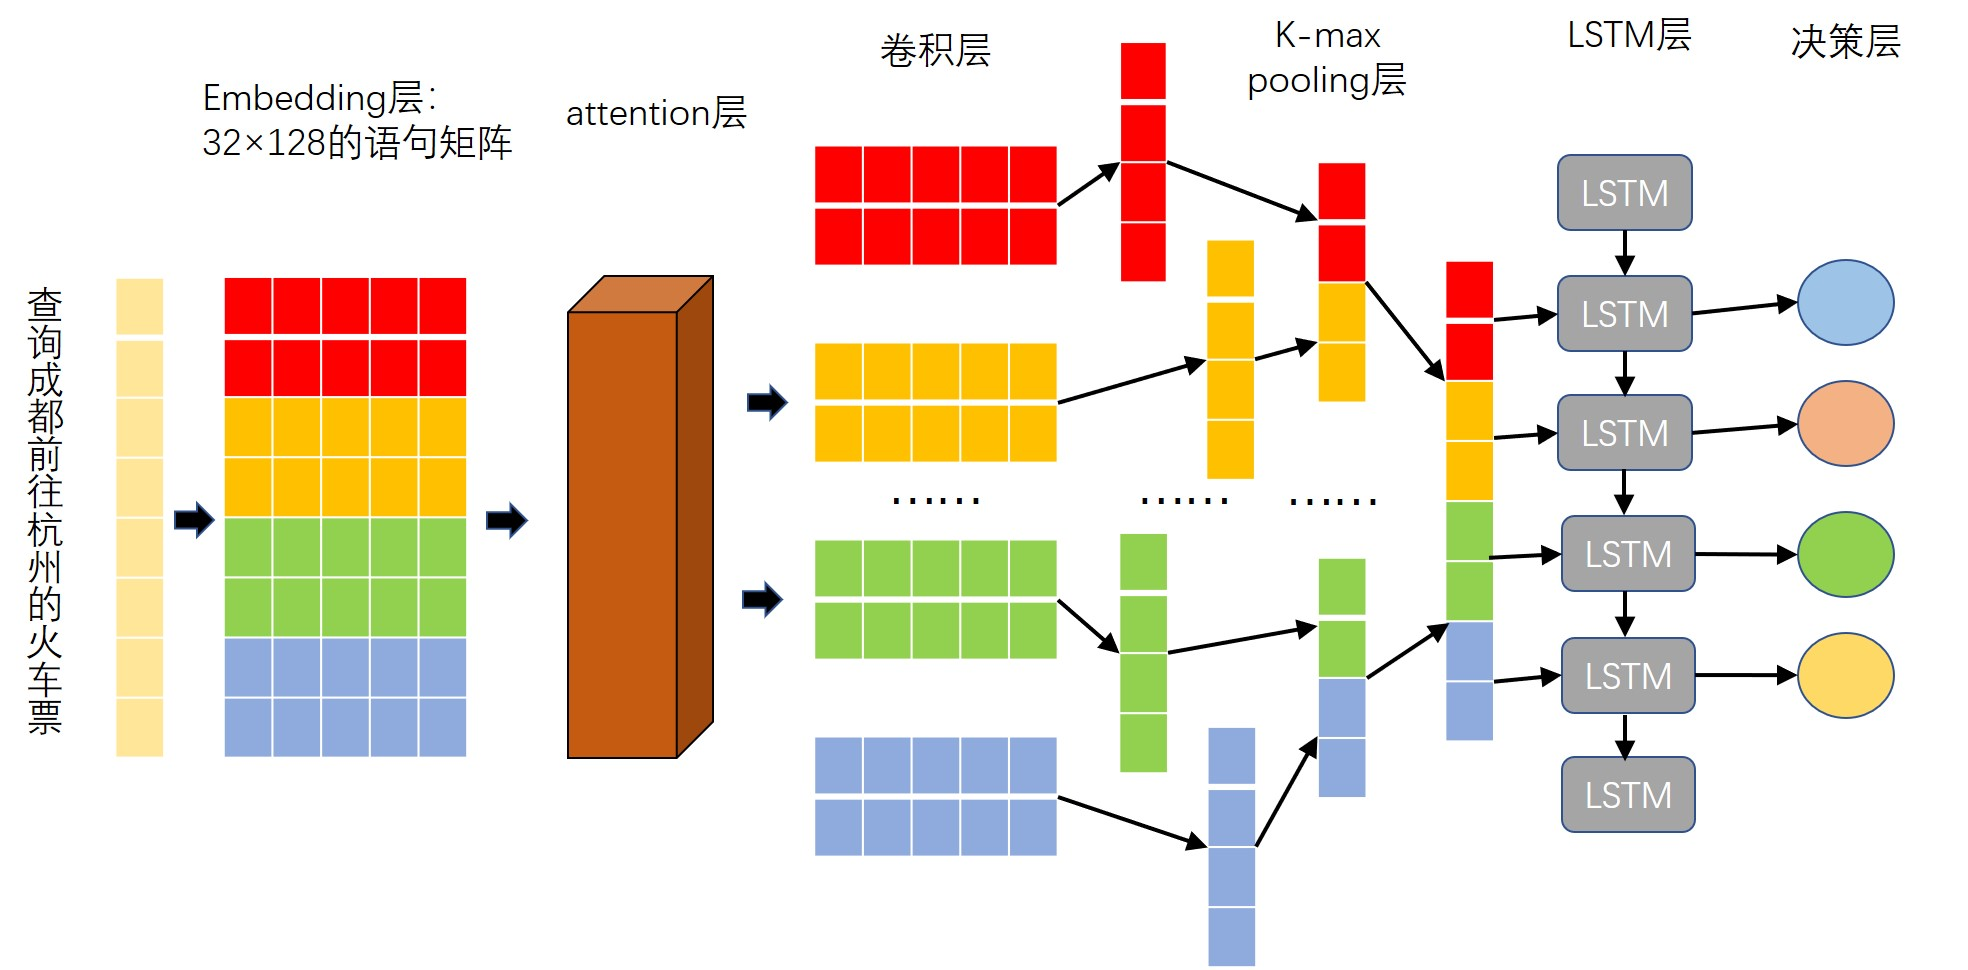
\includegraphics[scale=0.5]{./images/cnn-lstm.jpg}
    \caption{服务分类模型}
    \label{fig:cnn-lstm}
  \end{figure}


  \begin{figure}[htbp]
    \centering
    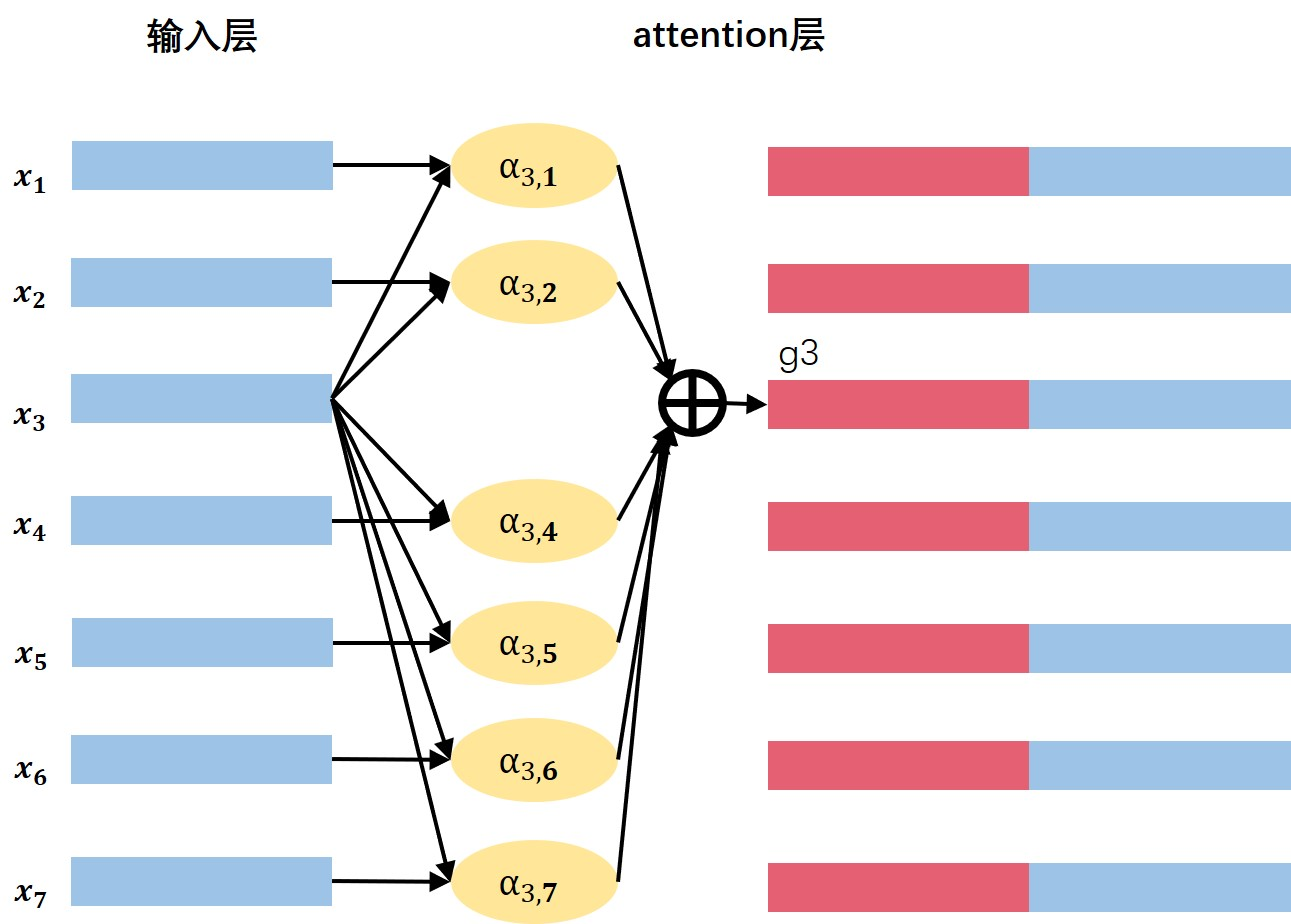
\includegraphics[scale=0.5]{./images/attcnn.jpg}
    \caption{服务分类模型中attention层}
    \label{fig:att-cnn}
  \end{figure}


  1)输入层与embedding层

  用户输入的语句通过结巴分词工具得到中文词的模型即可完成输入层的任务到达embedding层。之后将文本序列转换为矢量形式的数字表示,word2vec是最常用的方法之一。
  在本实验中,我们选择通过C-BOW模型基于维基百科中文语料库预训练得到的word2vec模型,通过使用预训练词向量模型可以有效地减少人工神经网络的过度拟合。
  由于神经网络的输入长度在本模型中是固定的,加之用户输入的语句长度通常有限,结合数据集中最长句子拆分以后的序列长度考量,我们决定把最大长度设为32.
  同时word2vec模型的输出的维度为128维,因此每一个需要匹配系统内服务的用户输入的句子就构成了一个32×128的二维矩阵E=[$e_{1}$,$e_{2}$,\dots,$e_{32}$],
  其中$e_{i}$=[$e_{i1}$,$e_{i2}$,\dots,$e_{i128}$]是一个中文词经过word2vec处理的向量表示。

  2)attention层

  如图\ref{fig:att-cnn}所示,是注意力层的主要结构,在输入层和卷积层之间引入了注意层.具体而言,注意力层是为每个词创建上下文向量。,
  上下文向量与词向量串联在一起,作为新的词表示形式将被输入到到卷积层。 凭直觉,一对彼此远离的词往往联系较少,因此,我们将距离衰减添加到注意力机制中。 
  注意机制的思想是在推导$x_{i}$的上下文向量$g_{i}$时将注意力集中在特定的重要单词上,图\ref{fig:att-cnn}中的红色矩形代表$g_{i}$。 
  注意机制是一个附加的多层感知器,它与ATT-CNN-LSTM的所有其他组件共同训练,这种机制确定了在预测服务类别时哪些词应比句子上的其他单词获得更多的关注。
  注意力机制生成的上下文向量$g_{i}$由一下公式得到:
  \begin{equation}
  \mathbf{g}_{i}=\sum_{j \neq i} \alpha_{i, j} \cdot \mathbf{x}_{j}
\end{equation}
其中,$\alpha_{i, j}$是注意力权值,其计算方式如下:
\begin{equation}
\alpha_{i, j}=\frac{\exp \left(\operatorname{score}\left(\mathbf{x}_{i}, \mathbf{x}_{j}\right)\right)}{\sum_{j^{\prime}} \exp \left(\operatorname{score}\left(\mathbf{x}_{i}, \mathbf{x}_{j^{\prime}}\right)\right)}
\end{equation}
\begin{equation}
\text { score }\left(\mathbf{x}_{i}, \mathbf{x}_{j}\right)=v_{a}^{\top} \tanh \left(W_{a}\left[\mathbf{x}_{i} \oplus \mathbf{x}_{j}\right]\right)
\end{equation}
词与词之间的score值由感知器计算得到,我们以此来度量词与词之间的相关性,得分越高表示相关性越强。
经过这一层的处理,用户输入的句子被转换为32×256的二维矩阵A=[$a_{1}$,$a_{2}$,\dots,$a_{32}$],
其中$a_{i}$=[$a_{i1}$,$a_{i2}$,\dots,$a_{i256}$]是一个中文词经过attention处理的向量表示。

  3)卷积层

  由于卷积核的存在,卷积层能够提取出词与词之间的隐藏的语义信息,捕获局部相关性。这里我们仅设置了单层的卷积层,用于捕获序列局部信息并对输入数据的降维。
  设置不同初始化权重的多个卷积核用于提高模型的学习能力,本模型共设置了64个卷积核,卷积核在文本矩阵上移动以提取特征。在文本处理领域CNN的卷积操作常被设置
  为一维卷积,这是因为直观上来看沿着词向量所在的维度不具有拆分性,因此卷积核总是沿着词与词之间的维度扫面提取特征,对m×n的矩阵以高为h的卷积核做一维卷积
  会得到一个高为m-h+1,宽为1的长条状矩阵。基于此,本文卷积核宽度与attention输出层
  一致为256,高度设置了[2,3,4]三种选择以期获得不同维度的语义信息,所以本层的输出结果大小随卷积核的尺寸不同会不一致,即会得到64个大小不一的矩阵称为feature maps.
  卷积操作的计算公式如下:
  \begin{equation}
    c=ReLU(W_{c}A+b_{c})
    \end{equation}
    这里选用ReLU作为非线性激活函数,可以改善网络的学习动态并显着减少深度网络中收敛所需的迭代次数,c为一个卷积核做一次卷积运算所得值。

  4)pooling层

    如上层所述,卷积层的输出结果大小随卷积核的尺寸不同会不一致,因此pooling层有统一维度的作用。
    同时可以降维降低计算复杂度,保留核心特征,减少模型参数防止过拟合提高模型泛化能力。
    由于卷积核卷积操作得到的结果是长条状,因此本文采用k-max pooling池化方法,k是超参数,设置为4.经过池化层处理后,得到4×64的特征矩阵作为lstm层的输入。
  
    5)lstm层

  直观上,文本分类是顺序信息处理的过程。但是,从卷积神经网络以并行方式获得的特征序列不包含序列信息,LSTM专为顺序建模而设计,
  可以进一步从CNN获得的特征序列中提取上下文信息,lstm内部核心计算过程如下:
  \begin{equation}
  f_{t}=σ(W_{f}\cdot[h_{t-1},x_t]+b_{f})
  \end{equation}
  \begin{equation}
    C_{t}=f_{t} * C_{t-1}+i_{t} * \tilde{C}_{t}
    \end{equation} 
    \begin{equation}
      o_{t}=\sigma\left(W_{o}\left[h_{t-1}, x_{t}\right]+b_{o}\right)
    \end{equation} 
    \begin{equation}
      h_{t}=o_{t} * \tanh \left(C_{t}\right)
    \end{equation}
    其中,$x_t$为从池化层输入的变量,其他字符代表的是lstm内部计算的中间过程变量不再赘述,得到的结果$x_t$被输入到下一层
  6)优化层与决策层


可以认为,矩阵分别经过卷积层和LSTM层后,可以获得高度提取的语义信息。


\section{基于的意图分类模型}